\chapter{Pointer and Effect Analysis}
\label{chap:pointer}
The problem of analyzing pointers is closely related to the field of effects
analysis. Indeed, establishing the relations between pointers require
understanding how and to what values fields are written to. Because of this
strong inter-dependence, it is often profitable to perform both simultaneously.

Our analysis builds summaries of methods, both in terms of effects and shape of
the heap. Those summaries are stored in graphs. In order that compute the
resulting graphs for each method, we perform a flow-sensitive
abstract-interpretation based analysis. A graph is thus associated to each
program point. The next section describes how those graphs are generated and
what their semantics are. This representation is similar in many aspects to
the graph representation used by Alexandru Salcianu in his Thesis. We can %FIXME
however point out two important differences: his work is primarily focused on
escape analysis, our isn't and thus we do not keep escape-specific information
in our abstract representation. We also introduced multiple kinds of global
nodes, that were not present in his work since it would be redundant for escape
analysis. Although the representations are similar, the semantics of our graphs
as well as the procedures to build them differ.

\section{Graph Semantics}
Our representation is based on labelled directed graphs augmented with some
metadata. They are defined by:
\begin{eqnarray*}
    G           := &\langle& N \subseteq Nodes, \\
                   && E \subseteq Edges, \\
                   && locVar \subseteq Variables \times \mathcal{P}(N), \\
                   && Ret \subseteq N ~ \rangle \\
    Edges       := && IEdges \cup OEdges  \\
    IEdges      := && \langle N, f, N \rangle \in Nodes \times Fields \times Nodes ~\textsf{ Inside Edges } \\
    OEdges      := && \langle N, f, N \rangle \in Nodes \times Fields \times Nodes ~\textsf{ Outside Edges } \\
    Variables   := && \textsf{All local variables and arguments} \\
    Fields      := && \textsf{Field names} \\
    Nodes       := && \{ GBNode, NNode \} \cup INodes \cup LNodes \\
                   && \cup PNodes \cup OBNodes \cup LitNodes \\
    INodes      := && \langle T \rangle \in TypeInfo \times ProgramPoints ~ \textsf{(Allocation node)} \\
    LNodes      := && \langle from, via, T \rangle \in Nodes \times Fields \times TypeInfo ~ \textsf{(Load node)} \\
    PNodes      := && \langle i, T \rangle  \in \mathbb{R} \times TypeInfo ~ \textsf{(Param node)} \\
    OBNodes     := && \langle T \rangle \in TypeInfo ~ \textsf{(Object Node)} \\
    LitNodes    := && \langle T \rangle \in TypeInfo ~ \textsf{(Literal values of primitive types)} \\
    NNode       := && ~ \textsf{(Null node)} \\
    GBNode      := && ~ \textsf{(Global node)} \\
\end{eqnarray*}

Nodes generally represent sets of objects (including literals of primitive
types), while edges represent may/must-point-to relations. $G$ also contains
$locVar$ which is a mapping from local variables to sets of nodes and $Ret$
consists of the set of nodes that are returned form the procedure.

We will present the abstract representations in a graphical manner. Instead of
attaching the metadata on the side, we will draw it directly on the graph using
the following convention: we draw local variables as shapeless nodes, with an
each to each node they point to, drawn in blue. Return nodes will be drawn
using double circle around nodes. Inside edges will be drawn using a full edge,
while outside edges will be dashed. To illustrate this, we represent in
Figure~\ref{fig:pt:graph1} a simplified graph corresponding to
\begin{eqnarray*}
    G &=& \langle \{n1, n2, n3 \}, \{ e1, e2, e3 \}, [ obj \mapsto \{n1\}, this \mapsto \{n2\}, tmp \mapsto \{ n1, n3 \} ], \{n3\} \rangle  \\
    n1 &:=& INode(T),~  n2 := PNode(0, T),~ n3 := LNode(n2, f2, T) \\
    e1 &:=& IEdge(n2, f1, n1),~ e2 := IEdge(n2, f2, n3) \\
    e3 &:=& OEdge(n2, f2, n3) \\
\end{eqnarray*}

\begin{figure}[h]
    \centering

    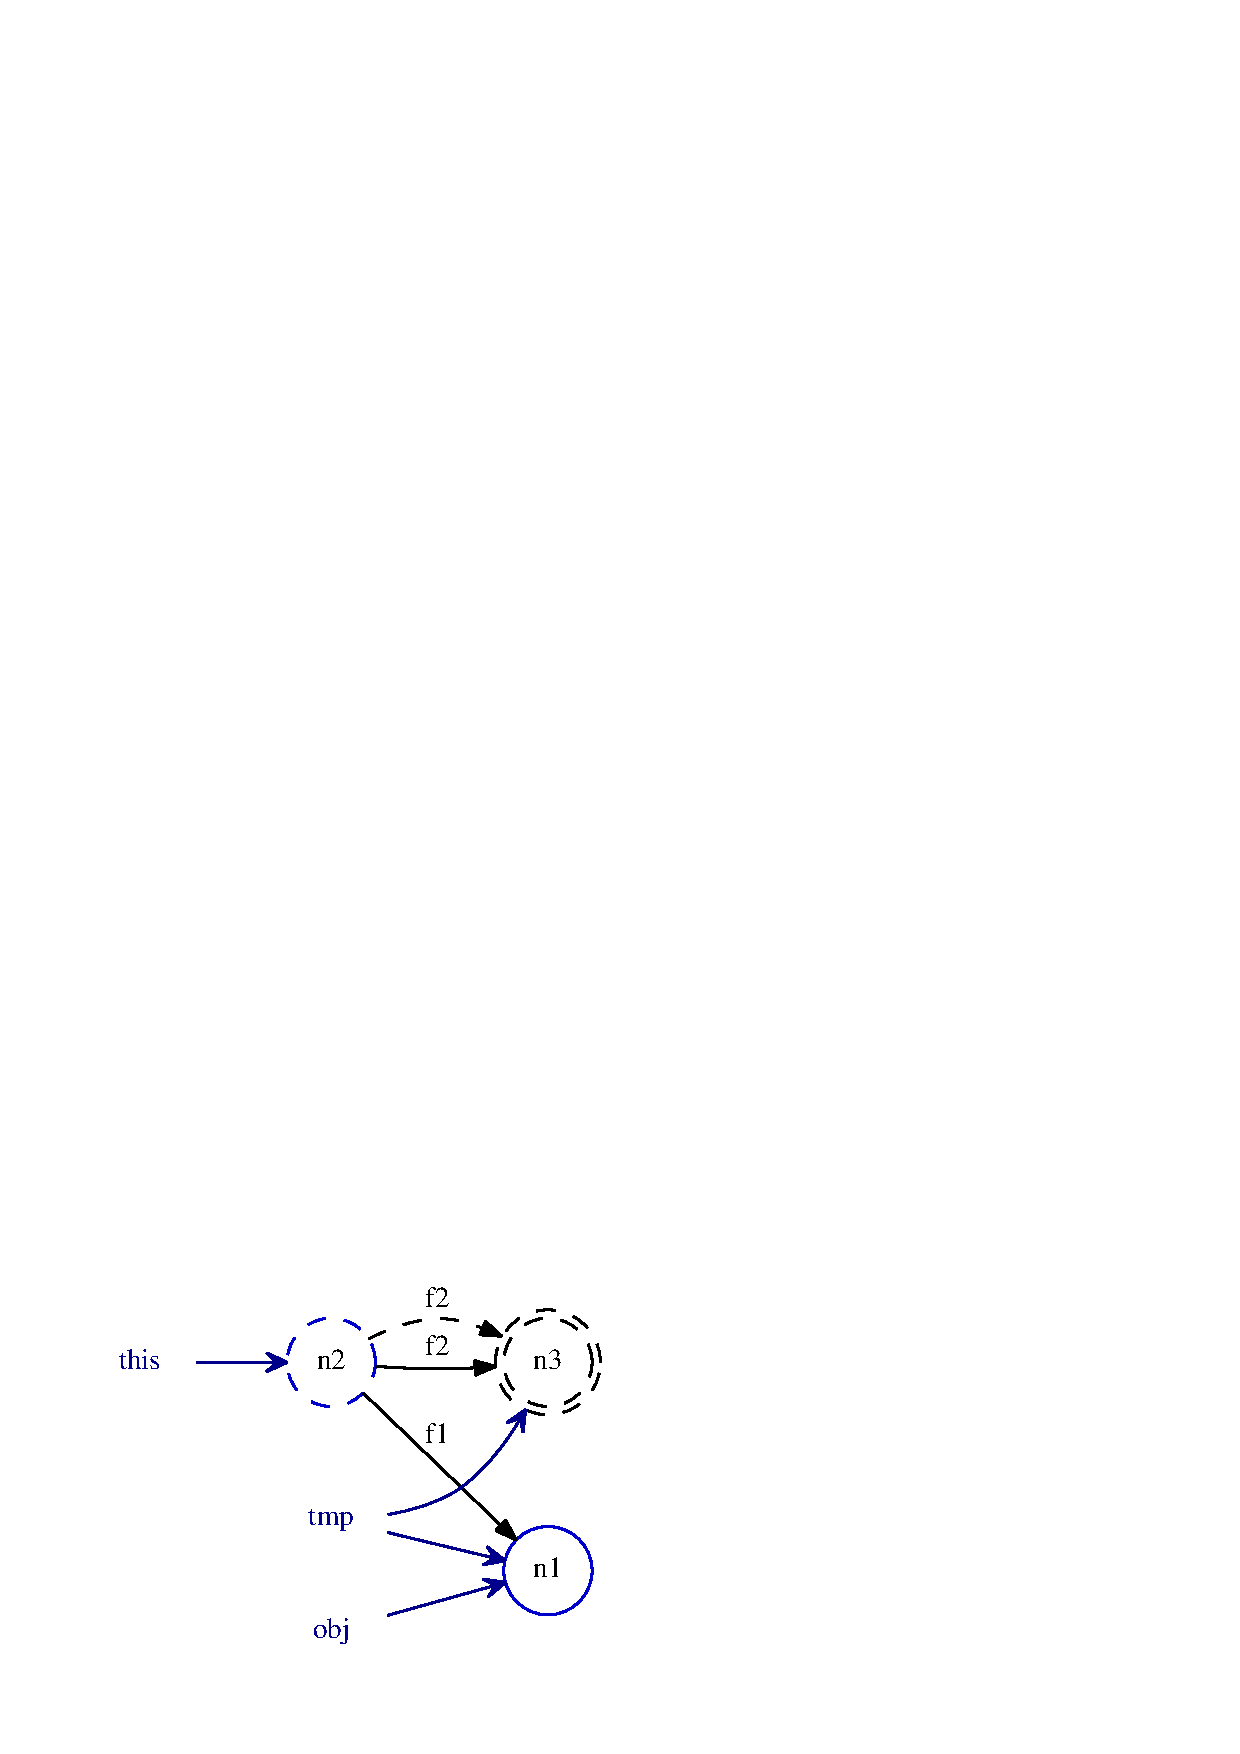
\includegraphics{images/pt_graph1}

    \caption{Simplified Graph Representation}
    \label{fig:pt:graph1}
\end{figure}

\subsubsection{Nodes}
As stated earlier, nodes represent sets of objects. Independently of their
kind, each node carry two pieces of information:
\begin{itemize}
    \item The type information $TypeInfo$, corresponding to the runtime types
    of the objects represented by the nodes.
    \item A \emph{singleton} flag, indicating whether the node represents only
    one object or may represent more than one. For instance, an allocation in a
    loop will yield multiple objects at the same allocation site.
\end{itemize}
We now quickly describe each kind of node and what their general meaning in a
graph is. Each kind of node will be accompanied with the actual graphical
representation, so that nodes are easily recognizable from the following
examples.

\paragraph{Inside Nodes}
Inside nodes (INodes) represent objects explicitely allocated via a \verb=new T=
statement. The graph will thus contain one \emph{INode} per allocation site.
The type of this node is exactly the allocated type (\verb=T=).
\begin{figure}[h]
    \centering

    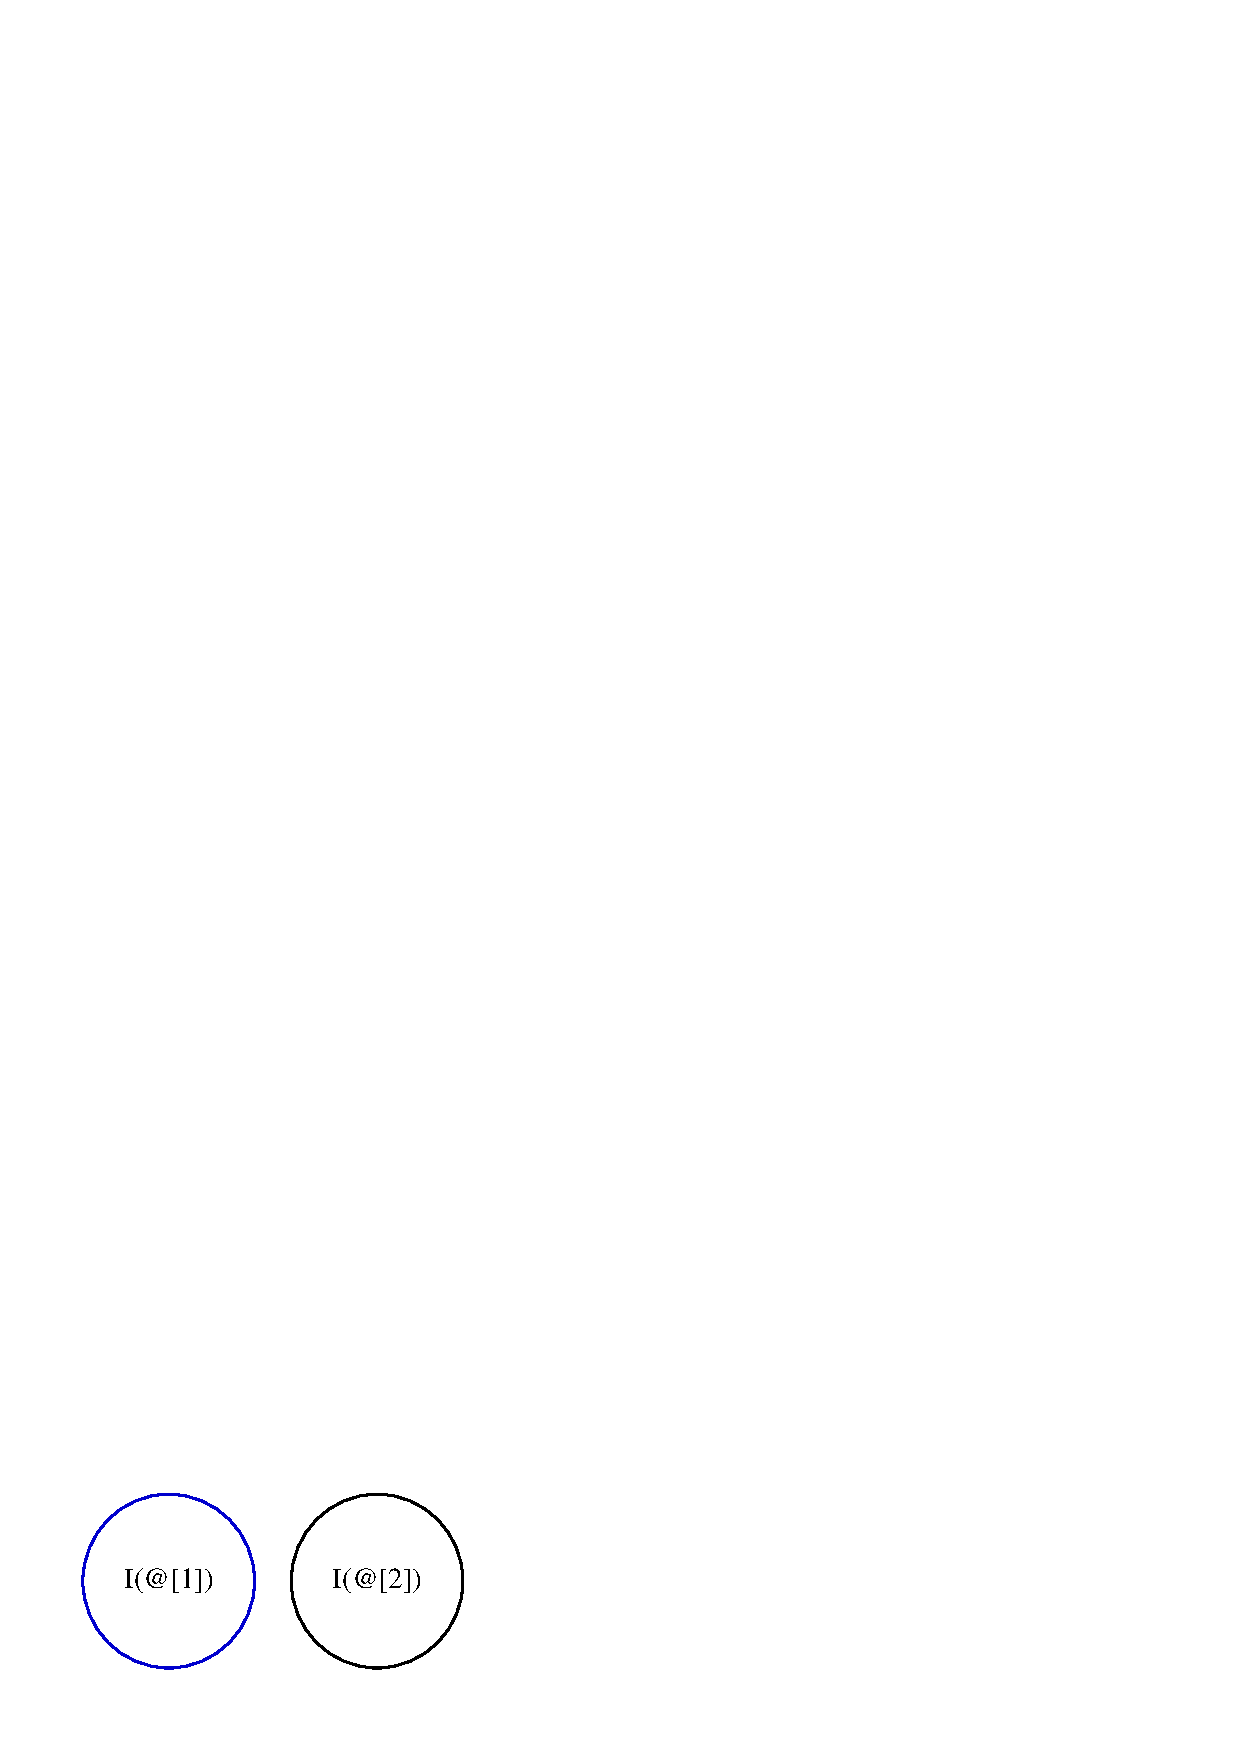
\includegraphics{images/pt_inodes}

    \caption{Two inside nodes at program points $@1$ and $@2$. Blue nodes are
    singleton objects.}
    \label{fig:pt:inodes}
\end{figure}

\paragraph{Load Nodes}
Intuitively, load nodes (LNodes) represent objects that are not yet determined.
For instance, the code:
\begin{lstlisting}
    def foo(arg: A) {
        val a = arg.f
        a
    }
\end{lstlisting}
will generate a load node representing the objects that \verb/arg.f/ points to
at the time of the call to \verb/foo()/. Section~\ref{sec:pt:inlining} will
describe in full detail how we resolve load nodes when inlining the graph of
the callee into the caller. We will not introduce load nodes if we don't have
to, for instance, in the following code:
\begin{lstlisting}
    def foo(arg: A) {
        arg.f = arg
        val a = arg.f
        a
    }
\end{lstlisting}
we know that \verb/arg.f/ points to \verb/arg/, and thus we don't need to
introduce a load node. Load nodes are conservatively assuming that they may
represent many objects, and their attached type is the compile type of of the
field and all its subtypes.

\begin{figure}[h]
    \centering

    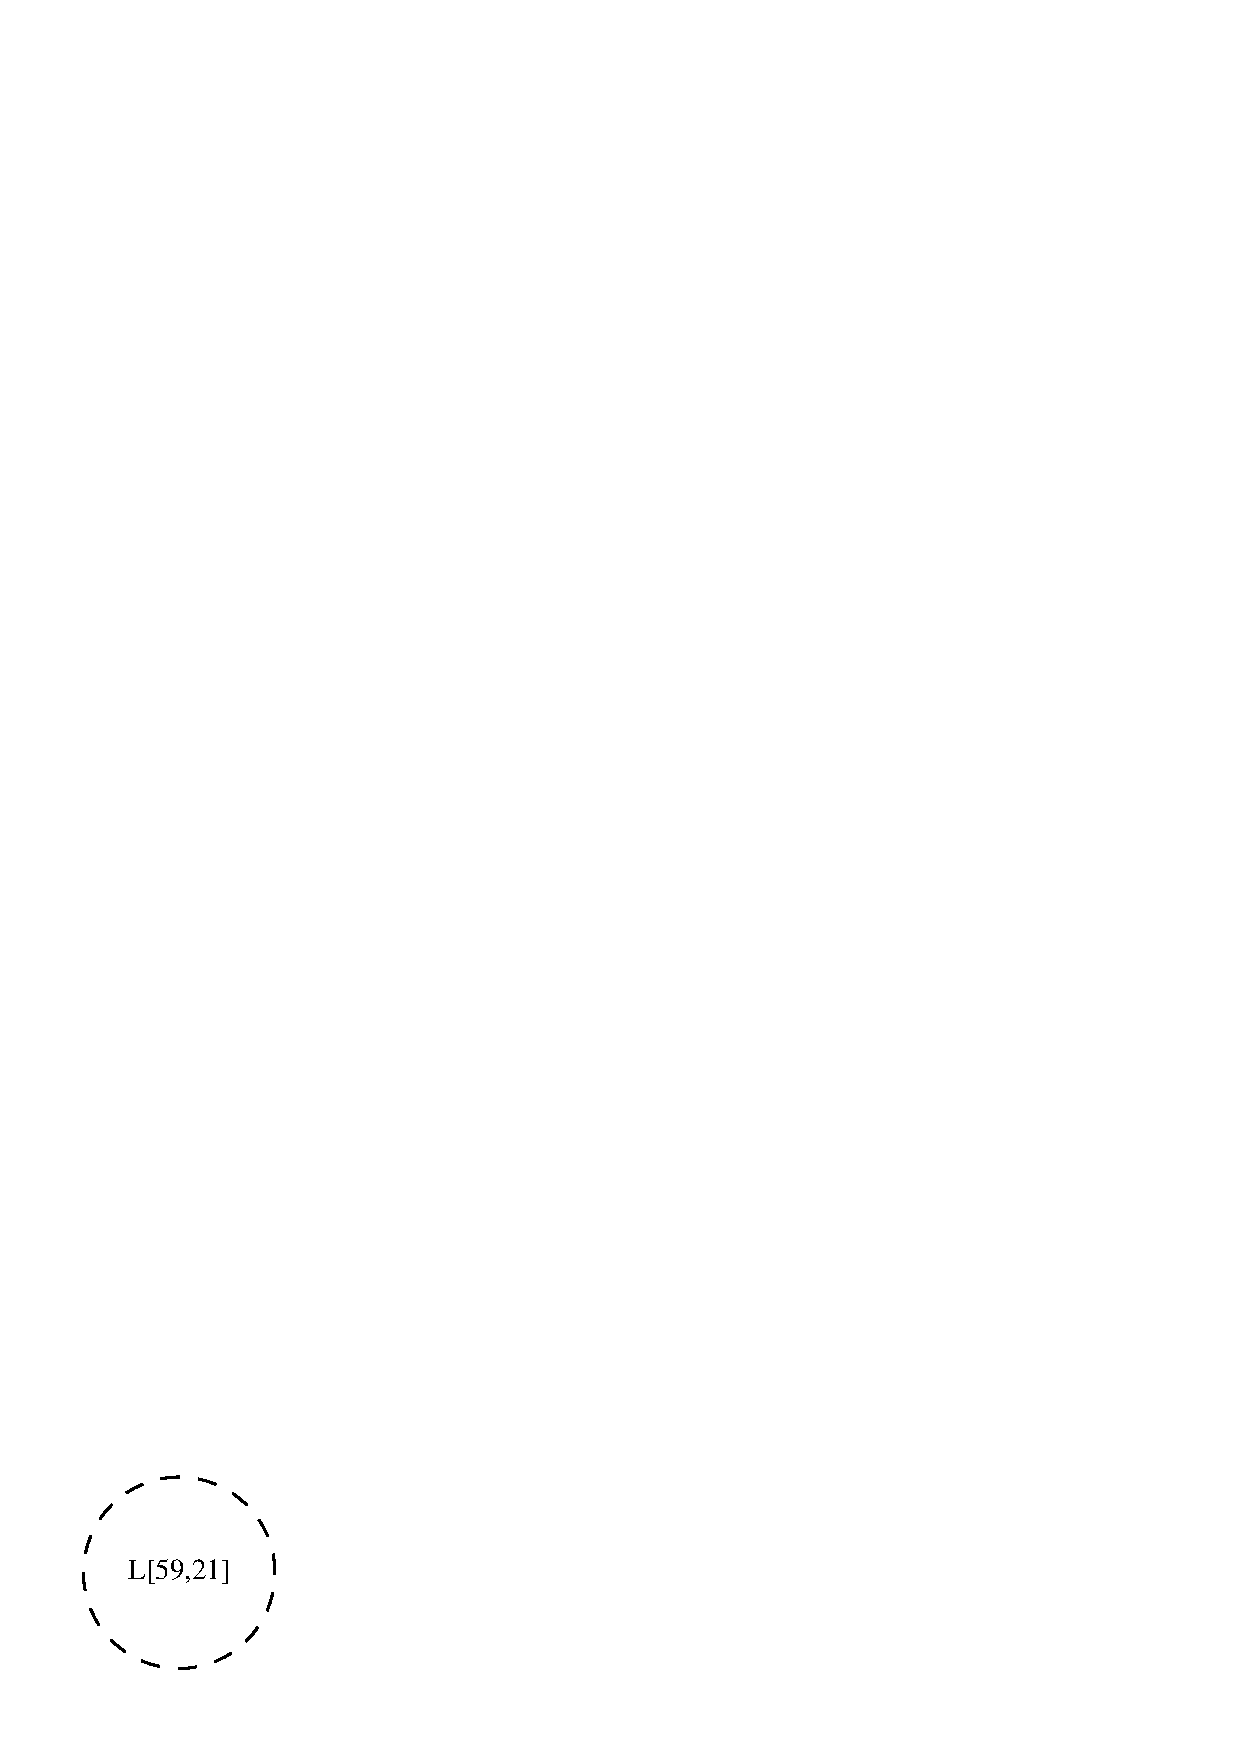
\includegraphics{images/pt_lnodes}

    \caption{Load Nodes are always dashed. Numbers used in the representation
    are used to uniquely identify them. Load nodes are never singletons.}
    \label{fig:pt:lnodes}
\end{figure}

\paragraph{Parameter Nodes} Parameter nodes (PNodes) represent arguments of the current
procedure. Parameter nodes are indexed by the position of the argument. The object
corresponding to the current instance ($this$) is implicitely defined as the
\emph{PNode} of index 0. For example, the following function definition:
\begin{lstlisting}
class A {
    def foo(arg1: B, arg2: C) // ...
}
\end{lstlisting}
will yield three (singleton) parameter nodes: $PNode(0)$ of type A and
subtypes, $PNode(1)$ of type B and subtypes and $PNode(2)$ of type C and
subtypes.

\begin{figure}[h]
    \centering

    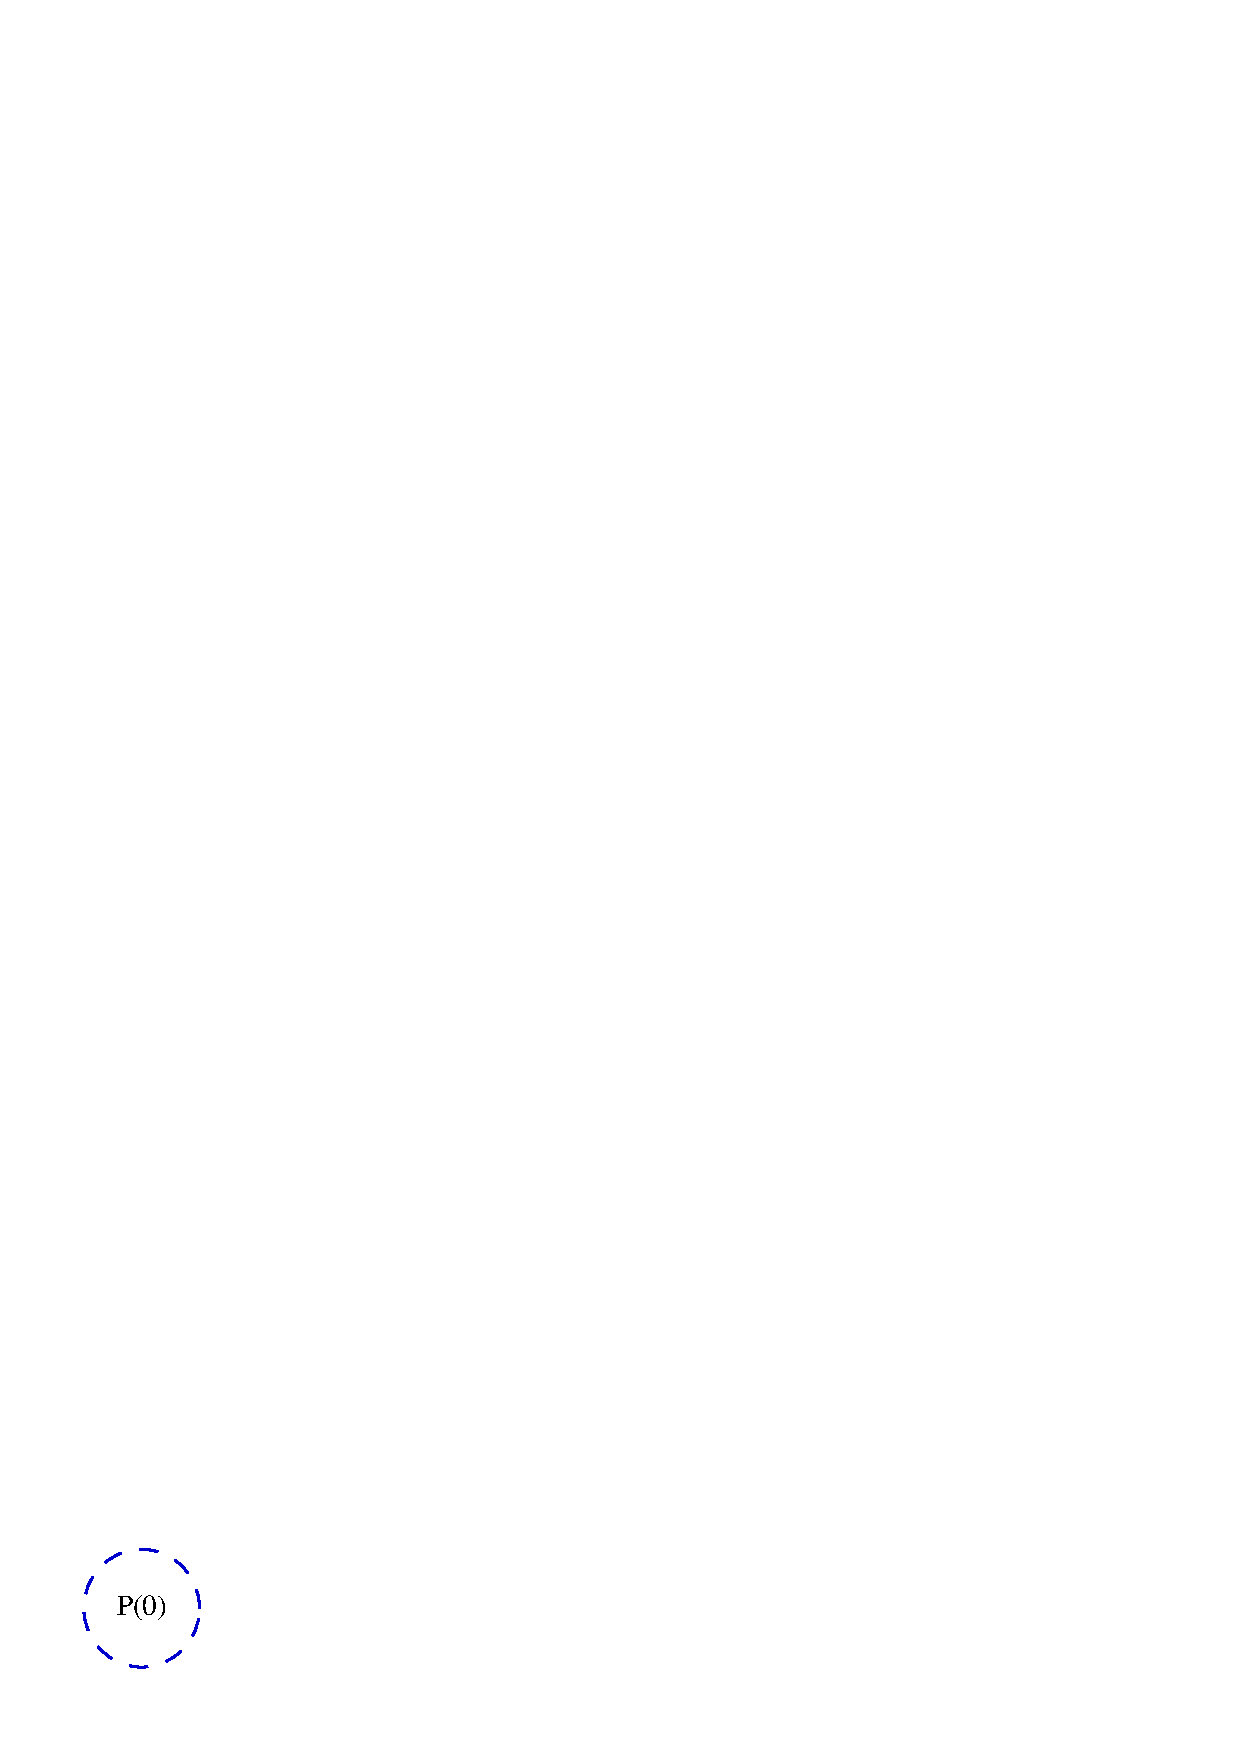
\includegraphics{images/pt_pnodes}

    \caption{Representation of a parameter node. They are always dashed and
    considered as singletons.}
    \label{fig:pt:pnodes}
\end{figure}

\paragraph{Object Nodes} Scala provides an elegant way of defining singletons
using the $object$ keyword. Object nodes (OBNodes) represent each of those
global singleton objects. Naturally, they represent a single object, and their
type information is exactly the type of the singleton.

\begin{figure}[h]
    \centering

    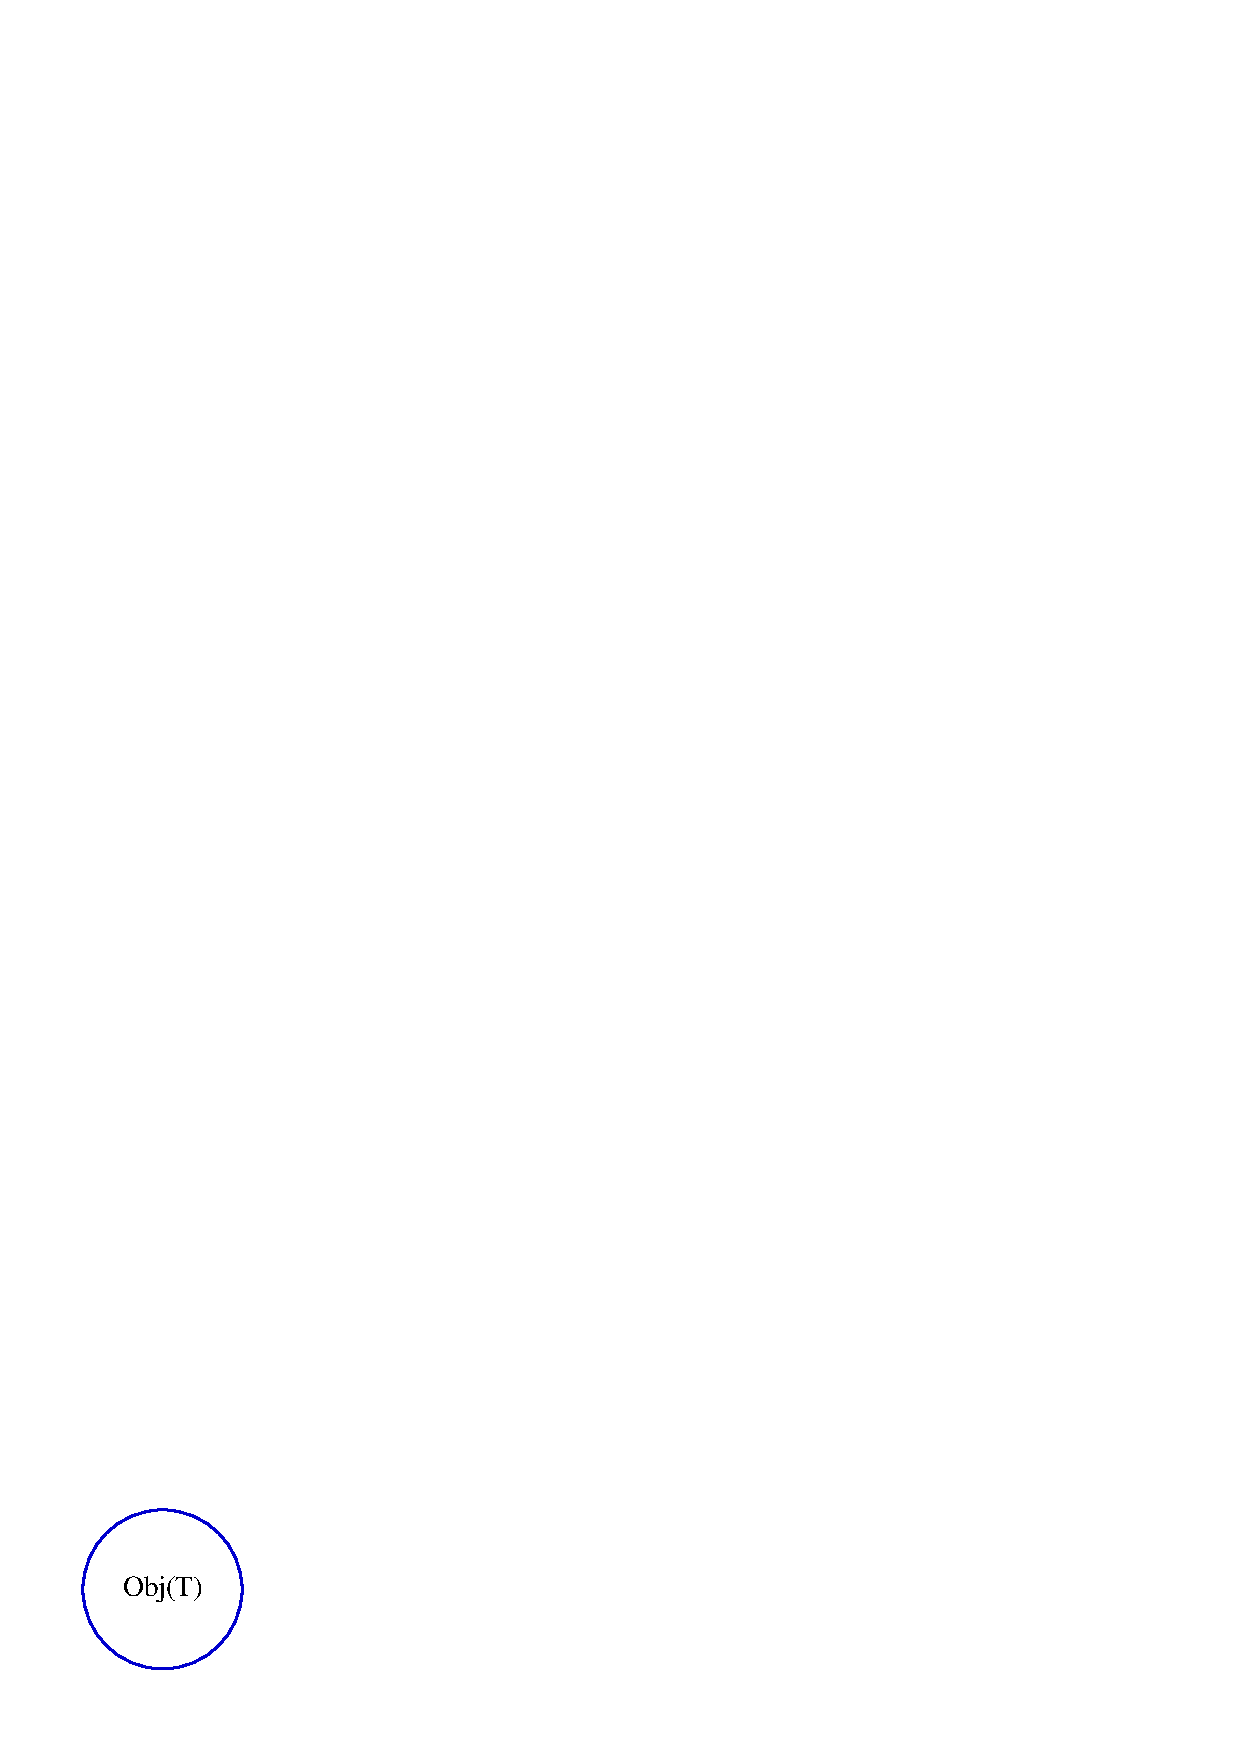
\includegraphics{images/pt_obnodes}

    \caption{Representation of a object node, always singleton.}
    \label{fig:pt:obnodes}
\end{figure}

\paragraph{Global Node} The global node (GBNode) represents all possible nodes,
it is thus of type \emph{Object} and subtypes, and is not singleton. This node
is seldomly used in error cases, and is similar to some \emph{havoc} operation.

\begin{figure}[h]
    \centering

    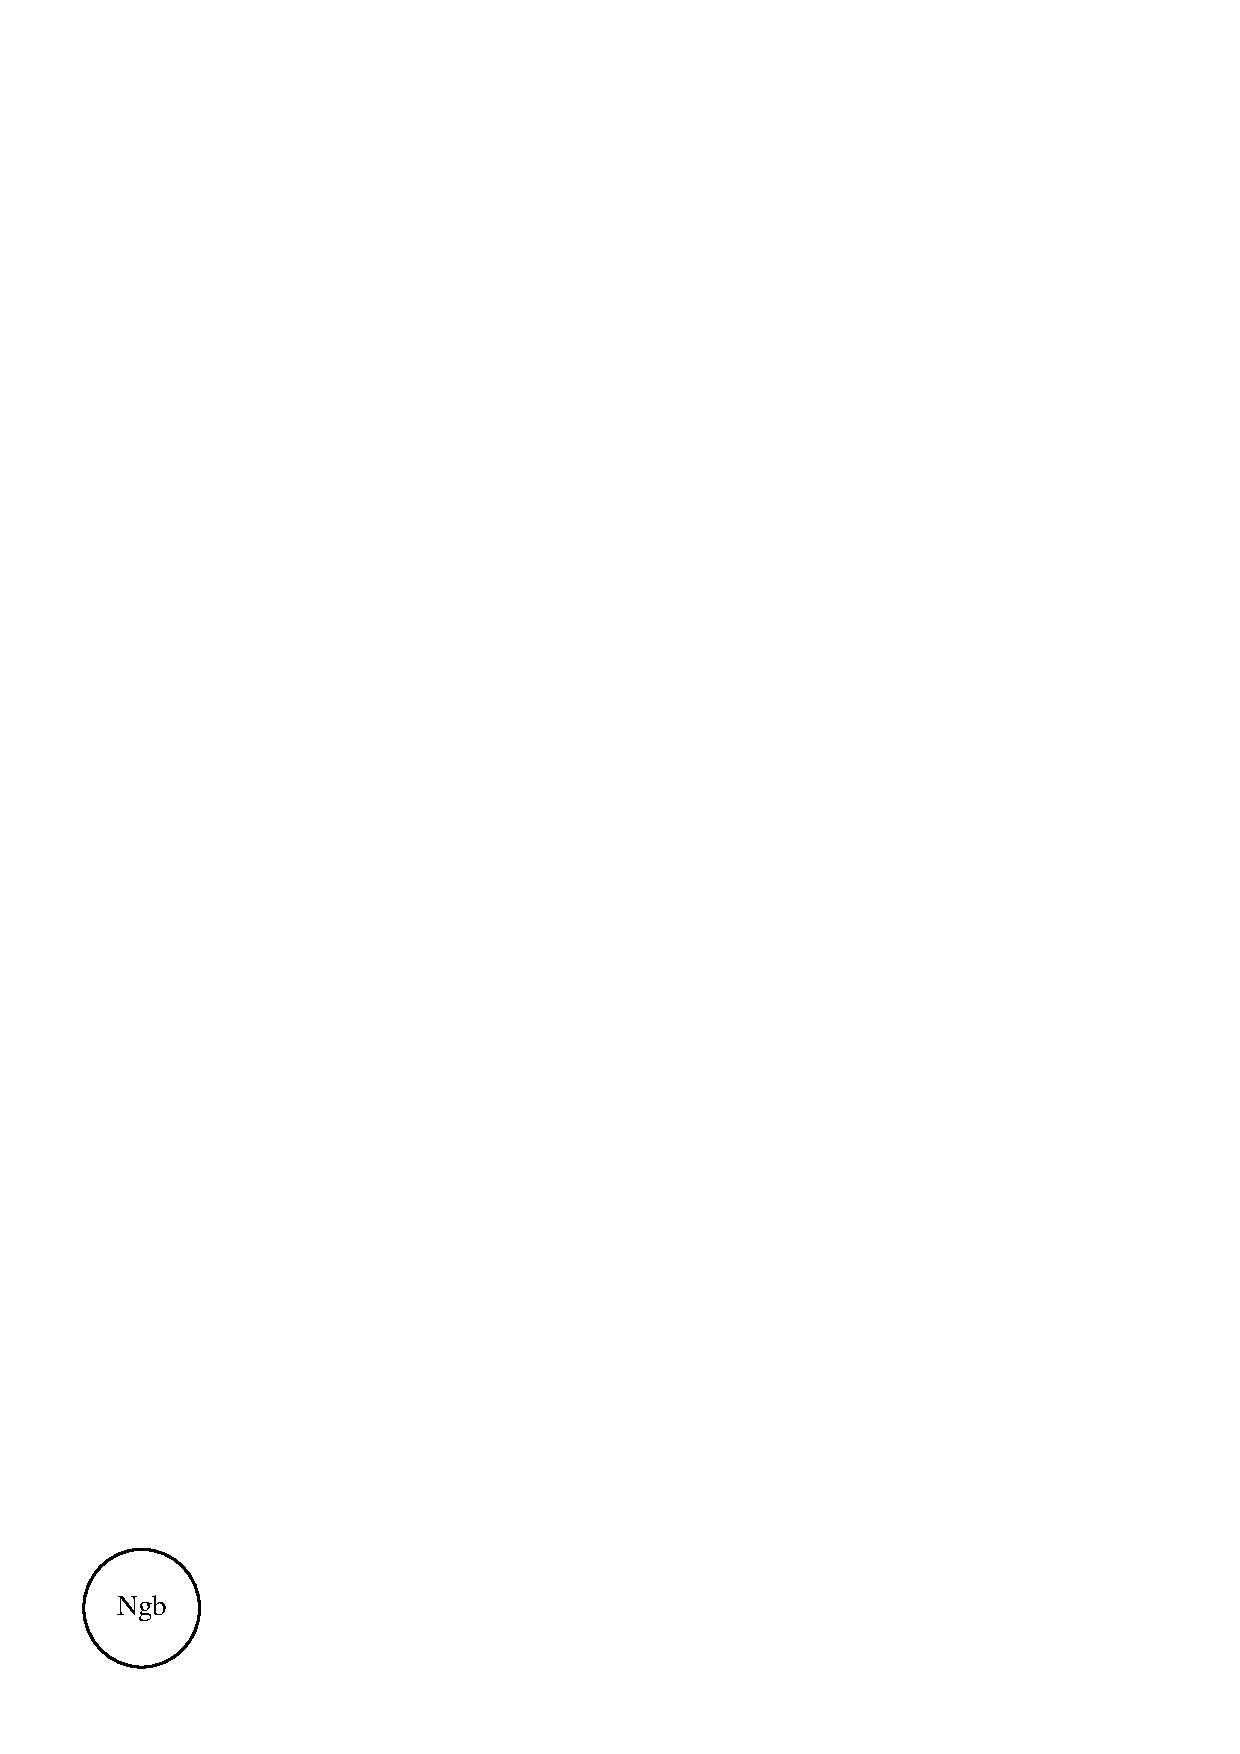
\includegraphics{images/pt_gbnodes}

    \caption{Representation of a global node, of all types and never singleton.}
    \label{fig:pt:gbnodes}
\end{figure}

\paragraph{Literal Nodes} Literal Nodes represent the literal values used
within the code. Except for Strings, those values are not in fact objects.
They will thus not have any outoing edge, and are here solely to record effects
of non-object fields. Intuitively, literal node shold the type of the literal,
and are singletons. Even though they are considered as singletons, we group
every literals of the same type into the same node. The singleton flag has no
effect as there is no outgoing edges.

\begin{figure}[h]
    \centering

    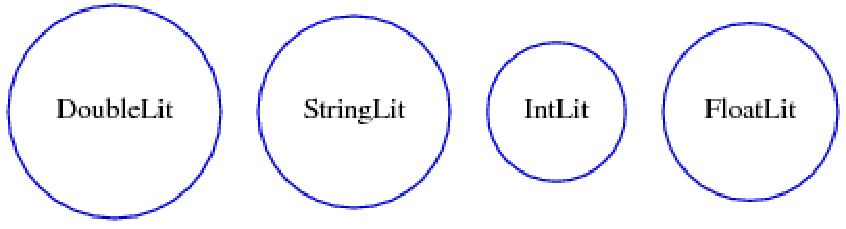
\includegraphics{images/pt_litnodes}

    \caption{Representation of some literal nodes, all singletons.}
    \label{fig:pt:litnodes}
\end{figure}


\paragraph{Null Node} The null node (NNode) represents the empty set of objects
corresponding to the $null$ value. It holds no type, and is considered singleton.

\begin{figure}[h]
    \centering

    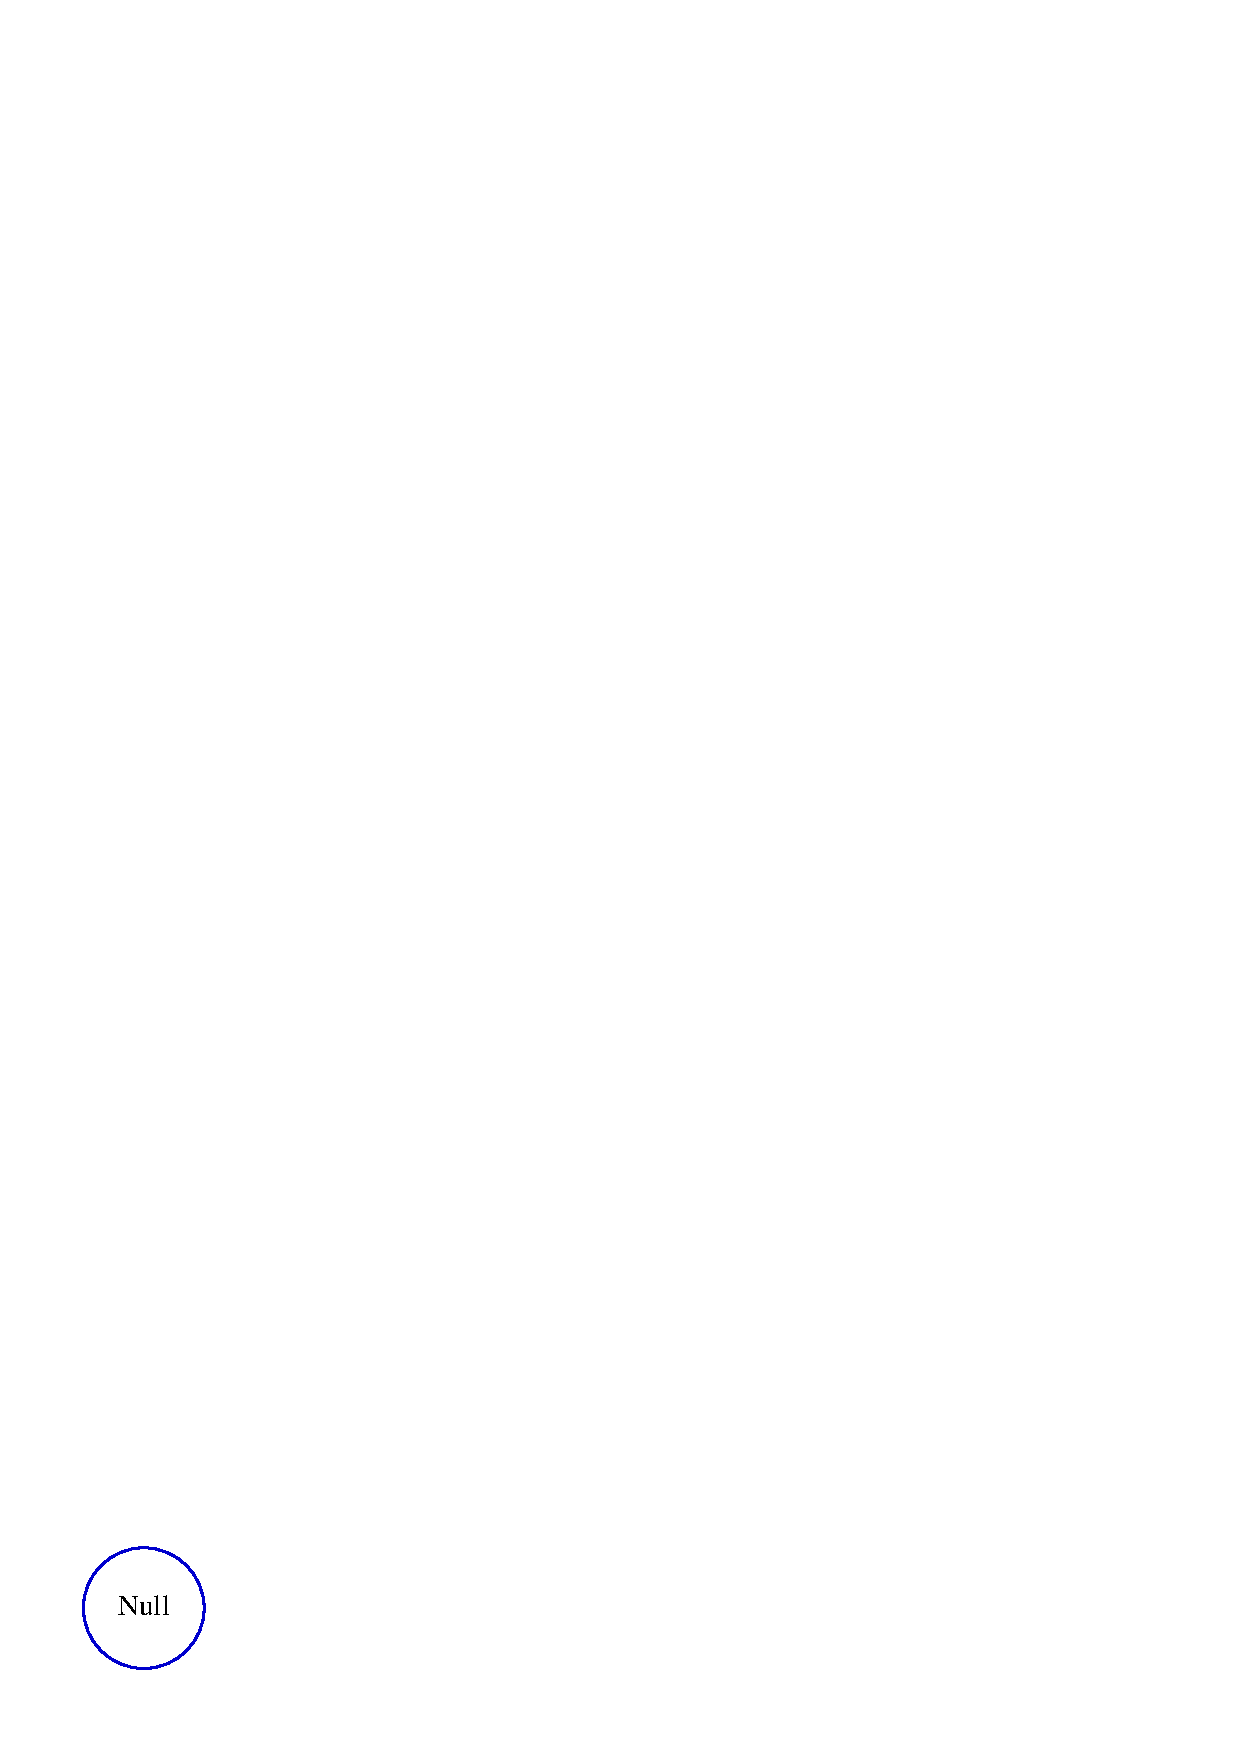
\includegraphics{images/pt_nnodes}

    \caption{Representation of a null node.}
    \label{fig:pt:nnodes}
\end{figure}

\subsection{Edges}
We distinguish two kinds of edges, \emph{inside} and \emph{outside} edges. We now
briefly describe what the meaning of each kind of edge is:

\paragraph{Inside Edges} Simply put, inside edges represent write operations to
fields. Inside edges are represented by a full arrow, labelled by the field on
which the write occurs. More than one inside edge with the same field can
originate from the same node.

\paragraph{Outside Edges} The intuition behind outside edges is that they
encode a way to reach load nodes. In other words, they represent a read on a
yet undetermined node. Outside edges are thus closely related to load nodes. In
fact, we have that every load node is reachable from a non-load node by
following outside edges only. Outside edges appear as dashed edges, labelled by
the field traversed.

To illustrate both kinds of edges, we consider in Figure~\ref{fig:pt:weak1} an
example of conditional update, along with parts of the resulting graph in
Figure~\ref{fig:pt:weak1graph}.

\begin{figure}[h]
    \centering
\begin{lstlisting}
class Plop(var next: Plop) {
  def test(a: Plop) = {
    if (a != null) {
      a.next = a
    }
  }
}
\end{lstlisting}
    \caption{Conditional update}
    \label{fig:pt:weak1}
\end{figure}

\begin{figure}[h]
    \centering

    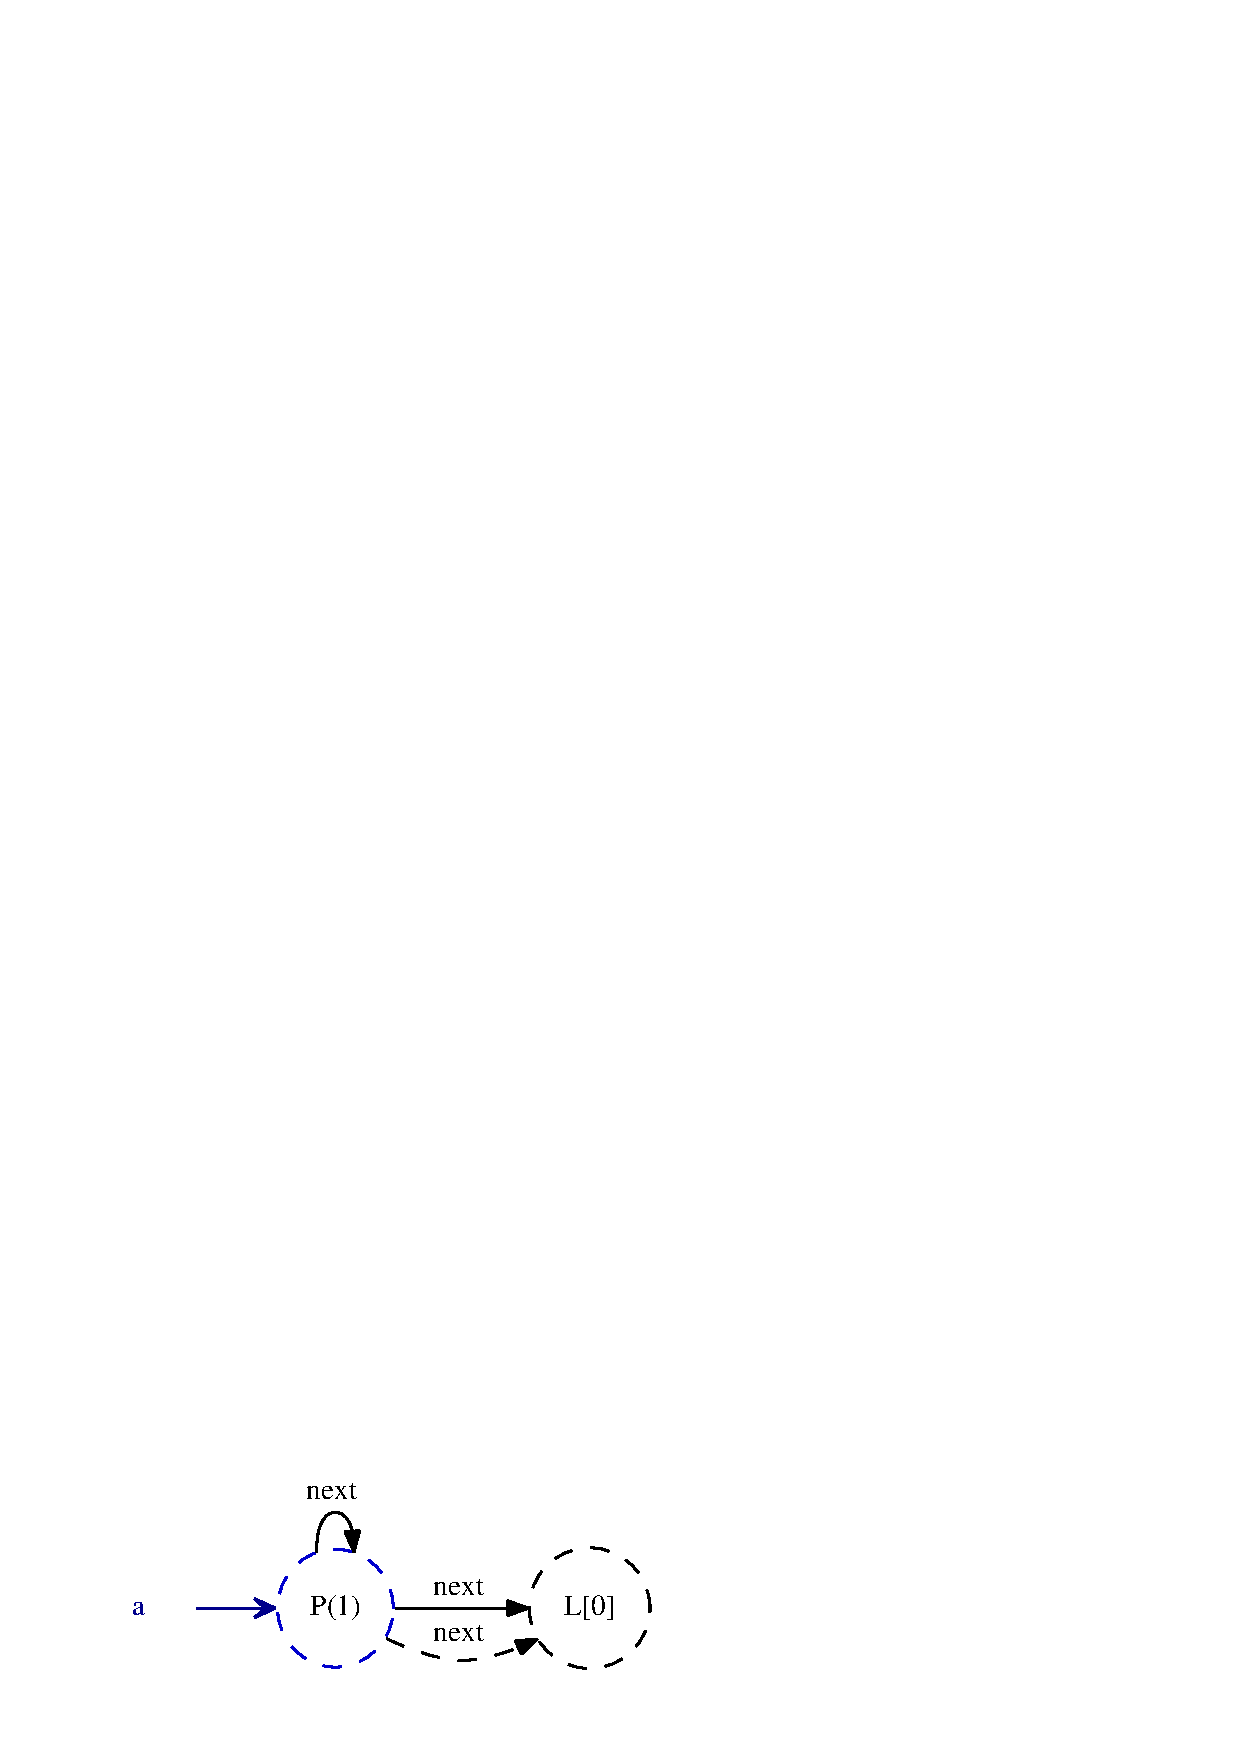
\includegraphics{images/pt_weak1graph}

    \caption{Graph with different kinds of edges, corresponding to the code on
Figure~\ref{fig:pt:weak1}}
    \label{fig:pt:weak1graph}
\end{figure}

After the call to this method, \verb/a.next/ either points to \verb/a/ or to
the old value, represented by the load node, which depends on the actual object
passed to \verb/test()/.

Now that graphs are better defined, we define some utility functions that will
be used thorough this report:

\begin{eqnarray*}
    nodes(G)(v \in Variable)  &:=& G.locVar(v) \\
    types(node \in Nodes)     &:=& node.types ~\textsf{(Type information attached to the node)} \\
    singleton(node \in Nodes) &:=& node.isSingleton ~\textsf{(Whether the node represents one object)} \\
    types(G)(v \in Variable)  &:=& \bigcup \{ types(node) | node \in nodes(G)(v) \} \\
    e.v1  &:=& ~\textsf{ The source node of the edge e} \\
    e.f  &:=& ~\textsf{ The field labelling the edge e} \\
    e.v2  &:=& ~\textsf{ The destination node of the edge e} \\
\end{eqnarray*}
We will usually omit specifying the graph $G$ if it is trivially inferred from
the current context.


\section{Weak and Strong Updates}
The concept of weak or strong updates relates to the possibility for an update to
discard old values. For example, after the execution of the following code:
\begin{lstlisting}
def test() = {
    val a = new Counter
    a.value = 2
    a.value = 3
}
\end{lstlisting}
the expected value of \verb/a.value/ is 3, and never 2. In this case, the
updates are \emph{strong}: they discard previously assigned values. However, in
the following code:
\begin{lstlisting}
def test() = {
    val a1 = new A
    val a2 = new A
    val a = if (..) a1 else a2
    a.value = 2
}
\end{lstlisting}
we know that \verb/a/ points to either \verb/a1/ or \verb/a2/. It would however
be wrong to assume that \verb/a1.value/ or \verb/a2.value/ is now exclusively
2. Generally speaking, we allow a strong update for $r.f = v$ whenever $r$
represents a single object. In more formal terms, we have that the condition
for a strong update on $r.f = v$ is:
$$
    (|nodes(r)| = 1) \land ( \forall n \in nodes(r).~singleton(n) )
$$

We also have to consider strong updates performed in a branch. Consider the
following code:

\begin{lstlisting}
def test() = {
    val a = new A
    a.f = 1
    if (..) {
        a.f = 2
        a.f = 3
    }
}
\end{lstlisting}

Even though some updates are conditional, we should be able to infer that
after the branch, the value of \verb/a.f/ is either 1 or 3, but never 2. We
will describe how branches are handled with respect to strong/weak updates in
Section~\ref{sec:pt:lattice}, describing the lattice and its join operation.

In case of a weak update, we can no longer discard the old value, and we will
still need to have an inside edge pointing to it. In case it is not yet
determined by the code, we introduce as usual a load node to represent this
previous value. This load node will then be mapped to the old value, as
described in Section~\ref{sec:pt:inlining}. Figure~\ref{fig:pt:weak1graph}
represents such a case.

In order to perform a precise alias analysis, it is key to be able to perform
strong updates as often as the code allows. It is evident that discarding old
values improves the overall precision of the analysis. For instance, without
any strong update, every object field would potentially still point to null,
which is the default value of every object field directly after the allocation
of the object.

\section{Join Operation}
We now describe the least upper bound ($\sqcup$). We generalize it to take an
arbitrary number of arguments $args := \{ a_1, ... a_n \}$. Intuitively, it is
the union of all graphs, with one exception regarding inside edges: if one node
present in all branches has an inside edge of a field originating from it in
only some of the branches, we will have to explicitely introduce a load node
along with its corresponding inside and outside edges. In other words, if one
branch performs a write on a field that is not determined in other branches.
\begin{eqnarray*}
    && \bigsqcup \{ \langle N, E, locVar, R \rangle \} := \langle N, E, locVar, R \rangle \\
    &&\bigsqcup \{ ..., \langle N_i, E_i, locVar_i, R_i \rangle, ... \} := \\
    && ~~~~ \langle \bigcup_i N_i \cup loadNodes, \bigcup_i E_i \cup loadEdges, \bigcup_i locVar_i, \bigcup_i R_i \rangle
\end{eqnarray*}
    where
\begin{eqnarray*}
    commonN &:=& \bigcap_i N_i \\
    allPairs &:=&  \bigcup_i \{ \langle ie.v1, ie.f \rangle | ie \in E_i \land ie \textsf { is IEdge}\} \\
    commonPairs &:=&  \bigcap_i \{ \langle ie.v1, ie.f \rangle | ie \in E_i \land ie \textsf { is IEdge}\} \\
    loadNodes &:=&  \{ LNode(p.v1, p.f) ~|~ p \in allPairs - commonPairs \land p.v1 \in commonN \} \\
    loadEdges &:=& \{ IEdge(in.v1, in.f, in) | in \in loadNodes \} \\
                 && \cup \{ OEdge(in.v1, in.f, in) | in \in loadNodes \} \\
\end{eqnarray*}

We now consider three code example illustrating the different cases. Each time
the graph of both branches will be provided, as well as the result of the join
operation on them.

\paragraph{Example 1}
Figure~\ref{fig:pt:join1code} contains a conditional update, without any previous
reference to the conditionally written field. This represents the corner case
in which we need to introduce a load node.
\begin{figure}[h]
    \centering

\begin{minipage}[t]{0.3\linewidth}
\vspace{0pt}
    \begin{lstlisting}
class A {
  var f: A = null
  def test(other1: A, other2: A) {
    if ( .. ) {
      this.f = other1 // Branch 1
    } else {
                     // Branch 2
    }
  }
}
    \end{lstlisting}
\end{minipage}

    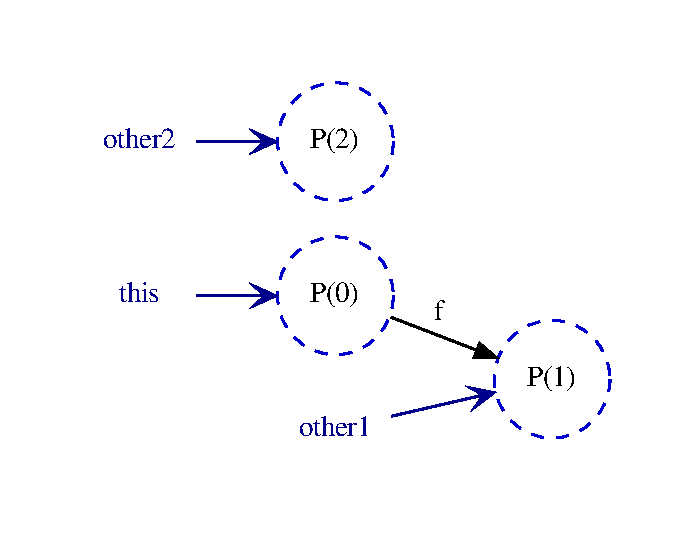
\includegraphics[scale=0.3]{images/pt_join1b1}
    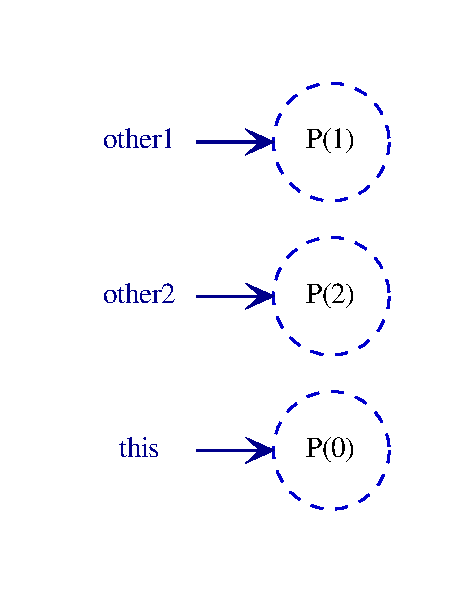
\includegraphics[scale=0.3]{images/pt_join1b2}

    \caption{Example 1: introduction of a load node}
    \label{fig:pt:join1code}
\end{figure}

\paragraph{Example 2}
Figure~\ref{fig:pt:join2code} contains a conditional update, preceded by a
write on the same field. In this case, no load node needs to be introduced.
\begin{figure}[h]
    \centering

\begin{lstlisting}
class A {
  var f: A = null
  def test(other1: A, other2: A) {
    this.f = other1
    if ( .. ) {
      this.f = other2 // Branch 1
    } else {
                     // Branch 2
    }
  }
}
\end{lstlisting}
    \caption{Code of example 2}
    \label{fig:pt:join2code}
\end{figure}

\paragraph{Example 3}
Figure~\ref{fig:pt:join3code} illustrate the case of a conditional write on the
same field with the same \emph{source} node, but with distinct destinations. We
are able to establish that after this conditional update, $this.f$ no longer
retain its old value.
\begin{figure}[h]
    \centering
\begin{lstlisting}
class A {
  var f: A = null
  def test(other1: A, other2: A) {
    if ( .. ) {
      this.f = other1 // Branch 1
    } else {
      this.f = other2 // Branch 2
    }
  }
}
\end{lstlisting}
    \caption{Code of example 3}
    \label{fig:pt:join3code}
\end{figure}
\section{Transfer Function}
\section{Inlining Graphs}
\label{sec:pt:inlining}

\section{Graph-based Type Analysis}
Even though our global type analysis was flow sensitive, it suffered from
critical imprecision with respect to fields and arguments. For this reason, we
implemented a type analysis based on our graphs. The approach we took is to
attach type information to each node. Since nodes represent objects, this is a
sensible thing to do. The additional information we store alongside each node
is similar to what we used in our previous type analysis: $(T_{sub}, T_{ex})$
a pair of two sets of types $T_{sub}$ and $T_{ex}$ where $T_{sub}$ represents
the set of types from which we need to include subtypes, and $T_{ex}$.
The set of runtime types attached to each node is determined based on the node
types. Figure~\ref{fig:pt:types} illustrates the main cases. We then use those
types in order to compute the set of potential targets for a method call. Given
the call \verb/obj.foo()/, we obtain the set of runtime types corresponding to
\verb/obj/ as follows:
$$
    types(\verb/obj/) = \bigcup \{ \gamma(types(n)) ~|~ n \in nodes(\verb/obj/) \}
$$
we can then look for potential targets in the resulting set of types, similarly
to what we did in our previous type analysis. 

\begin{figure}[h]
    \centering

    \begin{tabular}{ l | l }
        Node Type & Types Associated \\
        \hline
        INode(A)           & $\langle \emptyset, \{A\}\rangle$ \\
        LNode(a, f)        & $\langle\{type(a.f)\}, \{type(a.f)\}\rangle$ \\
        PNode(arg)         & $\langle\{type(arg)\}, \{type(arg)\}\rangle$ \\
        OBNode(A)          & $\langle \emptyset,   \{A\}\rangle$ \\
        NNode              & $\langle \emptyset,   \emptyset \rangle$ \\
        GBNode             & $\langle\{Object\},   \{Object\}\rangle$ (all)\\
        Literal Nodes      & $\langle \emptyset,   \{type(Literal)\}\rangle$\\
    \end{tabular}

    \caption{Summary: types associated to each kind of nodes}
    \label{fig:pt:types}
\end{figure}

If we pessimistically consider that each field read yield a \emph{load node},
and that every arguments become \emph{parameter nodes}, this type analysis is
exactly as precise as the one described previously. The main improvements comes
from two sides:
\begin{itemize}
    \item In practice, not every field reads yield a load node, for instance, a
read performed after a strong update will only return the newly assigned value,
which might be of a more precise set of types.
    \item When inlining those graphs, parameter nodes are mapped to other nodes
at the call site, and load nodes are resolved, if possible. The natural
inlining of methods makes this type analysis context sensitive. 
\end{itemize}
We consider in Figure~\ref{fig:pt:precise} an example illustrating this
improvement in precision.

\begin{figure}[h]
    \centering
\begin{lstlisting}
class A {
  var f: A = null
  def setF(a: A) { f = a }

  def test(obj: A) {
    val a = new A
    a.setF(a)
    a.f.foo()
  }
  def foo() {
    println("A")
  }
}

class B extends A {
  override def foo() {
    println("B")
  }
}
\end{lstlisting}
    \caption{Improved type analysis}
    \label{fig:pt:precise}
\end{figure}

At the time of the call to \verb/a.f.foo()/ we have from the graph at that
program point that \verb/a.f/ is the \emph{inside node} corresponding to the
object from \verb/new A/. We thus obtain $\{ \{\}, \{A\} \}$ for \verb/a.f/ instead of
$\{ \{A\}, \{A\} \}$, which excludes $B.foo$ from the call.
